\chapter{作品概述}

\section{应用背景与研究意义}

\subsection{机构定向通信的身份管理需求}

由统一机构管理账号、岗位和设备身份的通信系统，一条消息往往同时受到接收权限和发送来源两类
约束。以设备管理为例，运维中心向受控终端下发配置指令时，不仅要把内容限定给目标终端，还要让
终端只接受其认可的运维身份。机构内部的定向文件投递、跨部门业务流转和来源受限的数据分发也有
相同特点：通信双方的身份都参与消息能否被处理的判断。

在传统消息系统中，公钥加密控制消息的接收权限，数字签名提供发送来源认证。证书和账号目录
将现实身份与密码密钥关联，签名对象和加密对象分别承载认证与保密信息。应用协议需要统一身份
字段、证书传递、签名覆盖范围和加密顺序，使接收权限与发送来源共同绑定到一条消息。由机构
统一管理的定向通信，因而需要将两项身份关系贯穿密钥分发、消息生成和接收处理。

身份基密码为机构已经建立的身份管理体系提供了另一种表达方式。Shamir提出以用户身份直接参与
公钥密码运算的设想后，身份基加密、分层身份基加密和身份基签名分别发展出面向加密、分层发钥和
来源认证的算法\cite{shamir1984,gentrysilverberg2002,hess2003ibs}。邮箱、机构账号或设备编号经
规范编码后即可作为密码输入，可信发钥机构负责核验现实身份并签发私钥。该机制适合具有明确管理边界的组织，发钥机构负责保护主私钥并管理身份私钥的发放流程。

\subsection{双向身份匹配与通信关系保护}

身份基匹配加密（Identity-Based Matchmaking Encryption，IB-ME）把上述双向身份条件纳入同一
密码功能。发送者以自身身份$s$和目标接收身份$r$生成密文；接收者持有身份$r'$的接收方密钥，并在
解密时指定自己认可的发送身份$s'$。只有$r=r'$且$s=s'$同时成立时，接收端才恢复消息。IB-ME
最初作为匹配加密在身份策略下的专门形式提出，用于在完成双向匹配的同时提供消息隐私、发送来源
认证和通信身份保护\cite{ateniese2019me}。

表~\ref{tab:identity-cases}列出双方身份的四种匹配情况，说明两项身份条件如何共同决定消息恢复。

\begin{table}[H]
\centering\small
\caption{接收身份与认可发送身份的匹配关系}
\label{tab:identity-cases}
\begin{tabular}{ccc}
\toprule
\rowcolor{black!8} 接收身份 & 认可的发送身份 & 处理结果 \\
\midrule
匹配 & 匹配 & 恢复消息 \\
匹配 & 不匹配 & 拒绝 \\
不匹配 & 匹配 & 拒绝 \\
不匹配 & 不匹配 & 拒绝 \\
\bottomrule
\end{tabular}
\end{table}

IB-ME把“谁可以接收”和“接收者认可谁发送”统一纳入密码算法的输入和处理规则。身份条件随密钥、密文和解密输入共同参与处理；当底层身份基加密
具备匿名性时，公开信道上的观察者也不能直接从密文读出目标身份。图~\ref{fig:application-background}
以机构运维为例说明这种关系。可信发钥机构核验并发放身份密钥，发送端和接收端分别表达对方身份，
公开网络只承载密文。

\begin{figure}[!htbp]
\centering
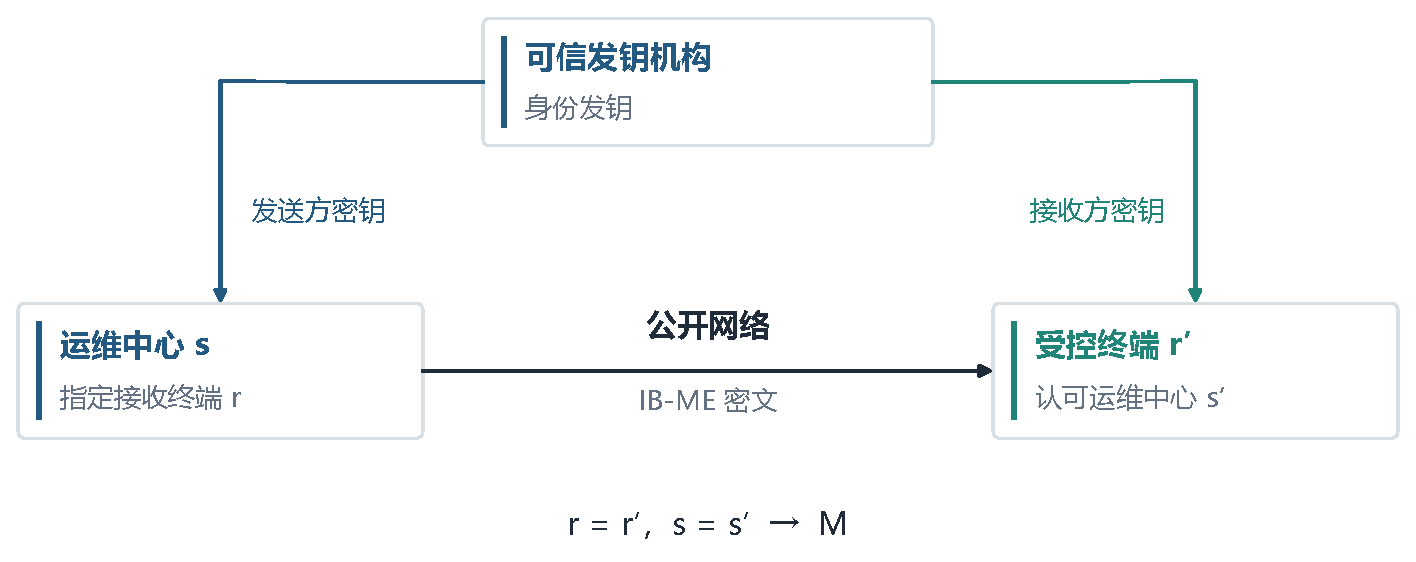
\includegraphics[width=\linewidth,height=.62\textheight,keepaspectratio]{figures/fig-01-01-roles.pdf}
\caption{机构定向通信中的身份与密钥关系}
\label{fig:application-background}
\end{figure}

这类能力能够对应到日常信息服务中的具体流程。例如，医院向患者发送检验报告或电子处方时，
内容只应由指定患者读取，患者端同时需要确认消息来自指定医院或医生；学校向学生、家长发送定向
通知时，接收者既要属于目标范围，也要确认发送方是相应学校或部门；智能设备接收配置或升级指令
时，设备身份与控制中心身份同样需要双向核对。它还可用于跨部门受控文件流转，以及原始IB-ME
研究讨论的隐私公告板等匿名而可认证的通信方式\cite{ateniese2019me}。这些应用模式共享双向身份
约束，但对在线延迟、密文长度、离线准备和连续通信成本的要求并不相同。因而，具体系统不仅需要
一个可运行的IB-ME方案，还需要根据使用方式选择和替换底层原语。

\subsection{后量子迁移下的格密码实现需求}

公钥加密和数字签名是上述通信机制的基础。当前广泛使用的RSA、Diffie--Hellman和椭圆曲线密码
分别依赖整数分解或离散对数问题。Shor算法表明，具备足够规模的通用量子计算机可以在多项式时间
内求解这两类问题\cite{shor1994}。对于需要长期保护的数据和生命周期较长的信息系统，密码迁移需要同步处理身份管理、协议组合、对象格式、运行资源和软件接入问题。

格密码以高维格上的计算问题为基础，是后量子公钥密码的重要技术路线。LWE、SIS及其环、模和NTRU结构变体能够支持加密、签名、身份基加密和身份基签名，并形成不同的实现路线。
矩阵与多项式表示、陷门形式、Gaussian采样和参数规模的差异，会直接改变密钥尺寸、密文长度、
运行时间和内存需求。这些原语进入同一软件时，需要统一接口、对象编码与调用规则。

因此，格上IB-ME的工程研究需要统一多类HIBE与IBS的协议接口，协调HIBE明文容量与签名、应用消息的长度，并降低结构化采样、对象编码和重复委派的成本。

\section{国内外研究现状}

身份基密码研究形成了加密、认证与匹配通信等多条支线。HIBE与IBS分别沿加密和认证方向发展，IB-ME研究围绕双向身份匹配、匿名性和认证模型展开；Wang等人的通用构造使这些支线在
两层匿名HIBE与IBS的组合处汇合。图~\ref{fig:research-timeline}按照原始论文的发表时间和技术关系
概括与本作品直接相关的研究节点与技术联系。

\begin{figure}[!htbp]
\centering
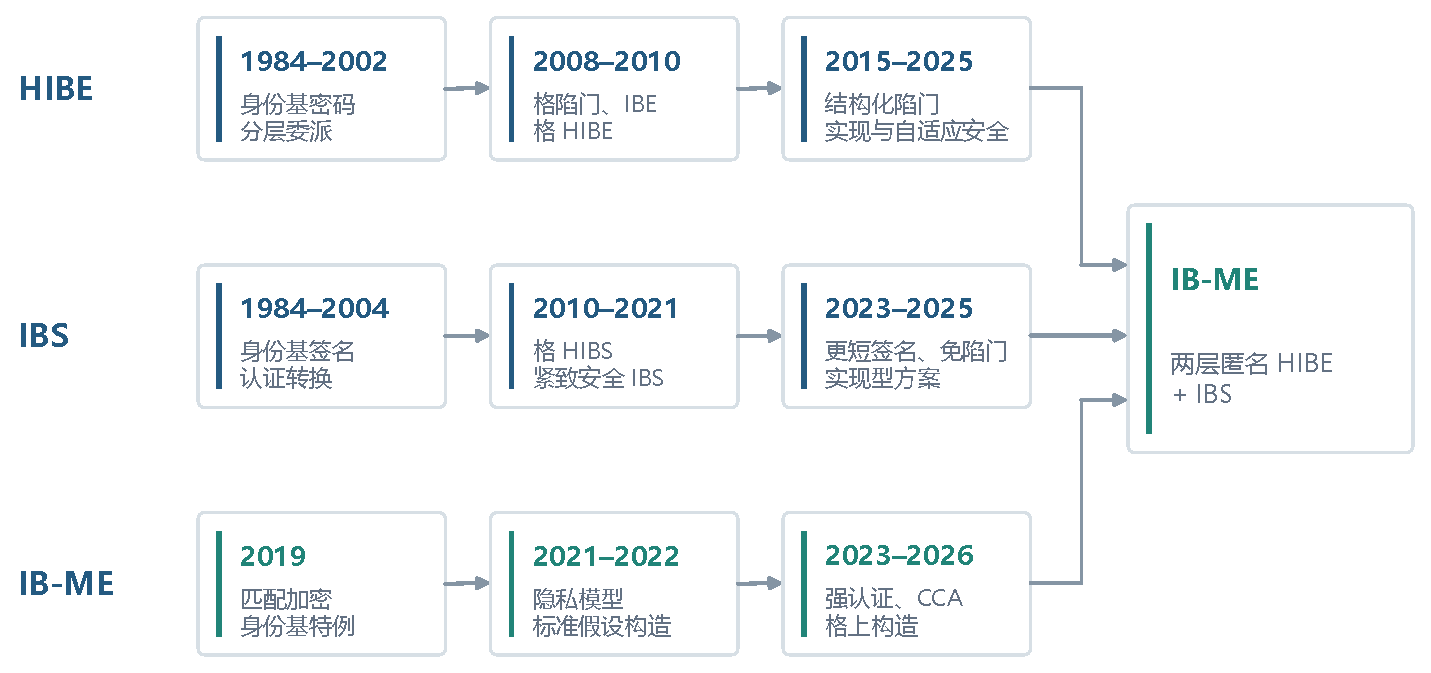
\includegraphics[width=\linewidth,height=.62\textheight,keepaspectratio]{figures/fig-01-02-research-timeline.pdf}
\caption{与本作品相关的三条研究支线及其汇合关系}
\label{fig:research-timeline}
\end{figure}

\subsection{身份基加密与分层委派的发展}

Shamir于1984年提出身份基密码的基本思想，但当时尚未给出完整实用的身份基加密方案
\cite{shamir1984}。Boneh和Franklin于2001年给出基于双线性对的IBE构造，使任意字符串作为加密
目标成为可实现的密码功能\cite{bonehfranklin2003}。Gentry和Silverberg随后提出HIBE，将单一发钥
机构扩展为分层体系：上层持钥者可以为下级身份委派私钥，而下级不能反向获得父级或兄弟节点密钥
\cite{gentrysilverberg2002}。这一变化使身份基加密能够对应机构、部门、岗位和设备构成的管理层级。

格上身份基密码的关键基础来自陷门和短原像采样。GPV工作在2008年给出格陷门、签名和匿名IBE
构造\cite{gpv2008}；Cash等人的Bonsai Trees以及Agrawal、Boneh和Boyen的两项工作在2010年把
格陷门委派用于HIBE，分别解决非双线性对HIBE、标准模型构造和委派后维度增长等问题
\cite{cash2010bonsai,agrawal2010hibe,agrawal2010delegation}。这些方案同时说明了格HIBE的主要
代价：身份深度、陷门表示与委派方法会影响私钥、密文和计算规模，委派算法的具体实现是影响运行成本的重要因素。

后续研究继续沿结构化表示和安全模型推进。Lai等人将Micciancio--Peikert型陷门扩展到理想格，
以环元素代替部分普通矩阵，并用于具有身份匿名性的（H）IBE\cite{lai2015trapdoors}。LATTE则面向
公开安全通信场景完成NTRU结构HIBE的系统化实现与评测，表明KeyGen、Delegate、Extract和
Gaussian采样是决定方案能否实际运行的核心环节\cite{zhao2024latte}。2025年的工作进一步推进了
标准假设下自适应安全和匿名HIBE的理论构造\cite{goyal2025adaptivehibe}。理论能力不断增强的同时，
具体方案在对象表示、委派成本和实现成熟度上的差异仍然显著，这也是本作品同时实现LATTE与Lai
两条HIBE路线的研究背景。

\subsection{身份基签名的格上实现路线}

Shamir在提出身份基密码时已经给出身份基签名（Identity-Based Signature，IBS）的设想。IBS
允许验证者使用签名者身份和系统主公钥验签。早期方案主要采用双线性对，例如Hess的身份基签名
构造\cite{hess2003ibs}。Bellare、
Namprempre和Neven随后形式化了认证转换：发钥机构为用户生成的普通验签公钥签发身份证书，用户
再用相应签名密钥签署消息\cite{bellare2004ibs}。这种路线能够复用成熟数字签名，但IBS签名需要
携带用户公钥、机构证书和消息签名；Galindo等人进一步研究了该转换对附加签名性质的适用范围
\cite{galindo2006ibs}。

格IBS的直接构造形成了另一条路线。Rückert于2010年给出格上层次身份签名，展示了陷门委派与
GPV型签名的组合\cite{ruckert2010hibs}。Pan和Wagner在2021年提出基于SIS与Ring-SIS的紧致安全
IBS，随后Sageloli等人简化参数和签名关系、去除一次昂贵的陷门委派，并给出具体参数
\cite{pan2021ibs,sageloli2023ibs}。这一路线使身份直接进入矩阵或环上的短向量关系，但陷门委派、
预像采样和大尺寸用户密钥仍会带来明显的时间与空间成本。

近年的工作进一步分化出不同工程取舍。Luo等人以两次Lyubashevsky型签名构造免陷门的模格IBS，
避免在发钥时进行格预像采样\cite{luo2024ibs}；SRGG将适合理想格IBE的预像采样与椭球
Gaussian形式的G＋G签名结合，并给出三组参数和概念验证实现\cite{jia2025ibs}。Wang等人还在
格上IB-ME研究中改进SIS型IBS，以缩短进入最终密文的签名\cite{wang2024ibme}。因此，认证转换、
矩阵SIS、模格和环格方案虽然都提供IBS接口，其发钥方式、签名计算、对象尺寸和内存需求并不相同；
通用组合设计通过独立后端管理这些特征。

\subsection{身份基匹配加密及格上构造的发展}

Ateniese等人在CRYPTO 2019提出匹配加密及其身份基特例，使发送端和接收端可以在不公开身份与
策略的条件下进行双向匹配\cite{ateniese2019me}。随后研究主要沿安全模型和构造基础两方面推进。
Francati等人在2021年研究无随机预言机的IB-ME并加强身份不匹配时的隐私描述
\cite{francati2021ibme}；Chen等人在2022年给出基于标准假设的构造\cite{chen2022ibme}。这些工作
仍主要依赖双线性群，因而尚未解决格上后量子实现问题。

Wang等人把发送消息的认证范围和自我伪造问题纳入更强认证目标，并提出由自适应安全的两层匿名
HIBE与IBS组成的通用构造。两层身份依次对应接收者和发送者，IBS为发送者生成的协议对象提供认证；
以格HIBE和格IBS实例化后，得到可抵抗量子攻击路线的IB-ME方案\cite{wang2024ibme}。这一构造
也是本作品公共协议的理论基础。其价值在于把HIBE和IBS的选择分离，其工程实现需要进一步统一软件对象、传输格式和容量规则。

2023年以来，相关研究又覆盖CCA隐私、标准格假设下的IB-ME以及标准模型中的格IBS与IB-ME
框架\cite{chiku2023ibme,belfiore2024ibme,yu2026ibme}。研究重点已经从“能否实现双向身份匹配”
扩展到不同隐私和认证目标、不同构造工具及后量子实例。与此相比，公开文献对多种目标参数HIBE、
IBS进入同一完整消息软件后的接口适配、状态保存、载荷组成和同机比较讨论较少。由此产生的具体
实现问题，构成下一节和本作品技术路线的出发点。

\section{现有研究的工程实现问题}

已有研究分别建立了分层身份加密、身份认证和双向身份匹配的理论工具，也给出了多种格上实例。
将这些原语组成支持应用消息、状态保存与后端替换的软件，还需要协调接口、对象与运行过程。本作品选取的具体方案在对象结构、明文容量、采样方法和状态生命周期上存在
明显差异，完整实现需要集中解决以下四类问题。

\textbf{原语接口和对象表示不同。} 本作品采用的HIBE与IBS分别使用矩阵、多项式、模向量和NTRU
对象，参数版本、身份映射、采样器和序列化方法也不相同。这些差异增加了统一接口、对象交换和
组合配置的实现难度。独立的后端接口将原语内部计算与公共消息流程衔接起来，为不同算法的配对
和扩展提供一致的调用方式。

\textbf{HIBE明文容量与IBS签名尺寸不匹配。} 部分HIBE只适合加密几十字节，而IBS签名可能达到
数KiB、数百KiB甚至更大，应用消息也没有固定长度。将“签名＋消息”直接作为HIBE明文，会使
不少组合超过容量上限。完整系统需要分离短秘密封装和大载荷加密，同时防止两部分被替换或重组。

\textbf{论文参数下的计算和存储开销较高。} 矩阵平方根、离散Gaussian采样和陷门委派若按稠密
矩阵直接实现，可能产生远超常规工作站容量的中间对象。通用JSON表示虽然便于调试，却会重复保存
大量整数的符号、分隔符和十进制字符。实现需要结合环结构、低秩分解和紧凑编码，降低中间对象
的存储与计算开销。

\textbf{连续消息服务的准备成本与在线成本不同。} 系统建立、用户发钥和固定身份对的叶密钥委派可以
被后续消息复用。长期密钥、会话叶密钥和逐消息对象具有不同生命周期，软件需要相应组织状态
保存与计算复用，并分别测量首次、重复和恢复后的运行成本。

\section{作品研究内容与技术路线}

本作品首先定义HIBE与IBS相互独立的后端接口，并依据两层匿名HIBE与IBS的通用构造实现系统建立、
发送方密钥生成、接收方密钥生成、消息加密和匹配解密五个公共算法。协议固定双方身份顺序和认证上下文，通过原语接口完成调用。

其次，作品实现LATTE、Lai两种HIBE，以及BNN＋ML-DSA、BNN＋Falcon、Luo、SRGG、Sageloli
五种常规IBS，形成十种端到端组合。另实现Wang--PW目标参数矩阵SIS后端，并完成其与LATTE的
完整消息流程。报告以“Wang--PW”表示这一具体IBS后端，并以Wang等人的通用构造建立公共IB-ME协议。

再次，作品针对实际运行中最突出的三类瓶颈完成Sageloli结构化环采样、SRGG范围感知编码和Lai
接收会话。三项工作分别减少大型中间矩阵、序列化空间和固定身份对的重复委派成本。

最后，作品建设规范对象、状态持久化、命令行和浏览器操作入口，并记录系统建立、双方发钥、首次
与重复收发、错误身份、密文篡改、对象尺寸和峰值内存。两种HIBE与五种常规IBS形成的十种组合
还在同一机器、输入和线程配置下完成基本性能比较，用于区分HIBE与IBS对协议各阶段的影响。
图~\ref{fig:work-overview}给出从底层原语到应用入口的总体技术路线。

\begin{figure}[!htbp]
\centering
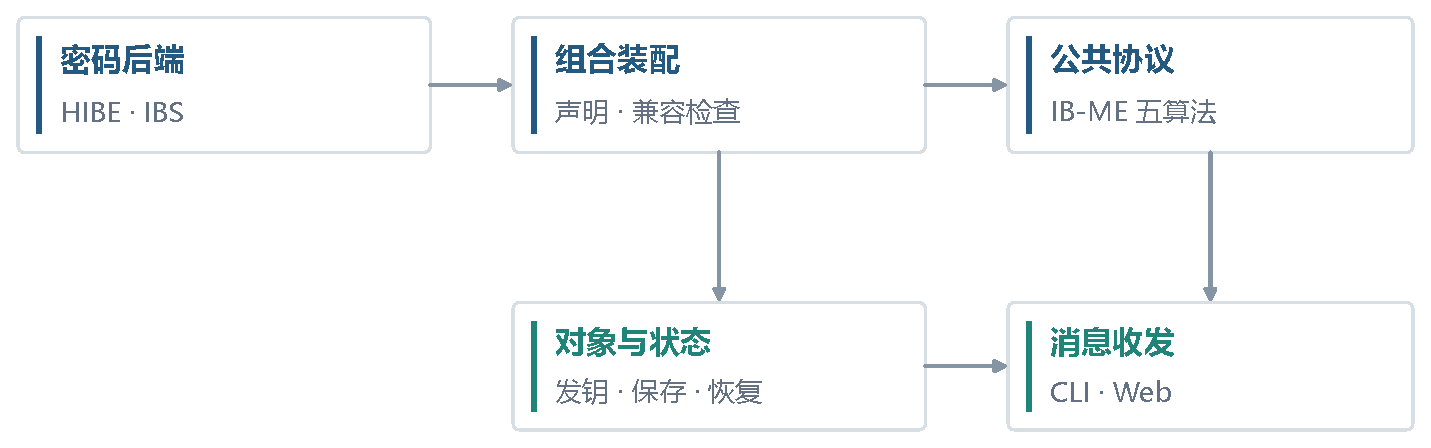
\includegraphics[width=.90\linewidth,height=.62\textheight,keepaspectratio]{figures/fig-01-03-roadmap.pdf}
\caption{作品总体技术路线}
\label{fig:work-overview}
\end{figure}

\section{主要工作}

本作品完成了从格密码原语、通用IB-ME协议到实际消息收发软件的完整系统。两种HIBE与五种常规
IBS形成十种组合，另接入LATTE＋Wang--PW目标规模组合。所有组合共用系统建立、双方密钥生成、
消息加密和匹配解密五个算法，并支持角色密钥保存、新进程恢复、命令行与浏览器操作。

\textbf{将目标规模环格采样组织为逐频率低秩计算。} Sageloli PARAM-I的相关扰动若展开为
$403456\times403456$双精度矩阵，单个矩阵的理论存储约为1.18~TiB。作品保留多项式表示，
在每个频率分解$65\times65$的Gram矩阵，完成PARAM-I、II的发钥、签名和公开验证；两组参数运行
实测峰值RSS分别约为1.36~GiB和6.19~GiB。

\textbf{用范围感知编码压缩原生IBS对象。} SRGG的公钥、机构状态、用户密钥和签名按字段取值范围
选择位宽，并采用规范二进制表示。三组参数中，机构状态长度降至对应JSON的18.3\%至19.8\%，
签名长度降至37.7\%至39.1\%；完整B组合采用紧凑签名格式。

\textbf{将固定身份对的委派移入接收会话。} Lai接收会话在准备阶段生成叶密钥，随后复用该密钥
处理连续消息。专项实验中，会话准备约510秒，后续解密中位时间由原路径的526秒降至28.6秒，
会话内解密提速约18.4倍、耗时减少约94.6\%。叶密钥编码长度为34.7~MiB。

十种常规组合在相同机器、源码、线程和输入下完成基本比较。表~\ref{tab:work-highlights}摘录
三组代表的在线收发指标；第七章给出全部组合、各阶段时间、对象长度和运行内存。

\begin{table}[H]
\centering\small
\caption{三组代表的同机在线收发结果}
\label{tab:work-highlights}
\begin{tabularx}{\textwidth}{@{}p{.30\textwidth}rrX@{}}
\toprule
\rowcolor{black!8} 代表组合 & 重复加密 & 重复解密 & 完整密文 \\
\midrule
A：LATTE＋ML-DSA & 13.5~ms & 59.4~ms & 139~KiB \\
B：LATTE＋SRGG & 11.3~s & 68.7~ms & 146~KiB \\
C：Lai＋Sageloli & 89.4~s & 409~s & 4.34~MiB \\
\bottomrule
\end{tabularx}
\begin{minipage}{.98\textwidth}\footnotesize
环境：Ultra~9~275HX，Sage~10.9，Python~3.13.14；双方身份各64~B，消息32~B。
每组1个独立系统，各项为固定密钥下第二次操作的实测值。C行采用逐次委派路径。
\end{minipage}
\end{table}

软件支持身份匹配、三类身份错配、密文字节篡改和对象恢复。十种组合共完成20次诚实加密、
30次诚实解密、10次新进程恢复和20次外层异常拒绝；网页提供消息发送、身份核对和解密结果查看。


\clearpage
\section{报告结构}

根据研究内容，本报告分为九章，具体安排如下。

\textbf{第1章\quad 作品概述：}介绍定向通信中的双方身份约束和抗量子密码迁移需求，梳理身份基加密、
身份基签名及匹配加密的发展脉络，分析多类格原语组成完整系统时面临的问题，明确作品的研究内容、
技术路线与主要成果。

\textbf{第2章\quad 基础知识：}介绍格、模运算、LWE与SIS及其结构变体，说明离散Gaussian分布、
格陷门和短原像采样的基本关系，解释环伴随、频域表示与低秩线性代数；给出IBE、HIBE、IBS与
IB-ME的定义、算法组成和安全目标，
建立后续方案设计所需的理论基础。

\textbf{第3章\quad 通用IB-ME系统设计：}说明系统参与方、密钥关系与双方身份的使用顺序，
给出各子算法的输入、输出和执行过程，设计短种子混合加密、发送身份认证与完整密文字节绑定，
并规定对象编码、状态保存和错误输入的处理方式。

\textbf{第4章\quad 算法实现与代表方案：}先列出已经完成的算法组合，再介绍两种HIBE与各类IBS的
关键计算、采用参数及原论文安全性依据。根据完整收发耗时、认证方式和连续通信能力，说明三组
代表的选取理由、性能取舍与典型应用场景。

\textbf{第5章\quad 关键算法优化：}围绕大规模采样内存、密钥与签名编码长度、重复委派耗时三个
瓶颈，分别展开Sageloli逐频率低秩采样、SRGG范围感知编码和Lai接收会话复用，解释计算方法、
数据组织及优化收益的来源。

\textbf{第6章\quad 软件系统与操作流程：}介绍软件分层、原语接口和组合配置，说明新增算法的接入、
身份密钥的保存恢复，以及命令行和浏览器中的系统建立、消息发送与匹配解密流程，给出软件运行
环境和部署方式。

\textbf{第7章\quad 测试与结果分析：}说明实验环境、输入和评价指标，比较十种组合的完整流程性能，
分析三组代表的计算、存储与通信成本，给出三项优化及Wang--PW组合的运行结果，并检验身份匹配、
篡改拒绝和状态恢复功能。

\textbf{第8章\quad 创新性与应用前景：}分别论述结构化环采样、范围感知编码和接收会话复用的技术
思路与实际价值，说明多算法系统的扩展能力，结合机构协作、终端指令和周期报送分析应用方式，
讨论算法迁移与业务系统集成。

\textbf{第9章\quad 总结与展望：}归纳通用系统、算法实现与性能优化的主要成果，结合实验结果总结
不同组合的计算和通信特点，从通信效率、算法扩展及长期身份管理等方面展望后续研究方向。
